\chapter{Einleitung und Zielsetzung}
\label{chap:Einleitung und Zielsetzung}
\section{Coole Einleitung}
\label{sec:Coole Einleitung}
Lorem ipsum dolor sit amet, consetetur sadipscing elitr, sed diam nonumy eirmod tempor invidunt ut labore et dolore magna aliquyam erat, sed diam voluptua. At vero eos et accusam et justo duo dolores et ea rebum. Stet clita kasd gubergren, no sea takimata sanctus est Lorem ipsum dolor sit amet. Lorem ipsum dolor sit amet, consetetur sadipscing elitr, sed diam nonumy eirmod tempor invidunt ut labore et dolore magna aliquyam erat, sed diam voluptua. At vero eos et accusam et justo duo dolores et ea rebum. Stet clita kasd gubergren, no sea takimata sanctus est Lorem ipsum dolor sit amet. Lorem ipsum dolor sit amet, consetetur sadipscing elitr, sed diam nonumy eirmod tempor invidunt ut labore et dolore magna aliquyam erat, sed diam voluptua. At vero eos et accusam et justo duo dolores et ea rebum. Stet clita kasd gubergren, no sea takimata sanctus est Lorem ipsum dolor sit amet.

Duis autem vel eum iriure dolor in hendrerit in vulputate velit esse molestie consequat, vel illum dolore eu feugiat nulla facilisis at vero eros et accumsan et iusto odio dignissim qui blandit praesent luptatum zzril delenit augue duis dolore te feugait nulla facilisi. Lorem ipsum dolor sit amet, consectetuer adipiscing elit, sed diam nonummy nibh euismod tincidunt ut laoreet dolore magna aliquam erat volutpat.

Eine Abbildung referenziert man so: Abbildung \ref{fig:bsp}

\begin{figure}[ht]
\centering
\caption{Hier ein Beispiel für das Einbinden einer Grafik}
\label{fig:bsp}
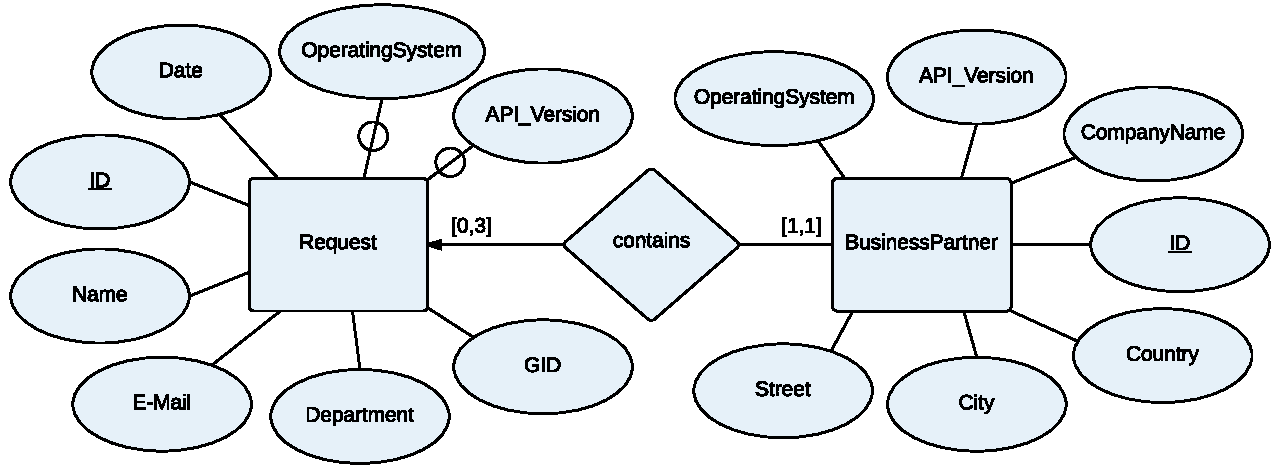
\includegraphics[width=0.8\textwidth]{\figdir/er-model.pdf}
\end{figure}

Ut wisi enim ad minim veniam, quis nostrud exerci tation ullamcorper suscipit lobortis nisl ut aliquip ex ea commodo consequat. Duis autem vel eum iriure dolor in hendrerit in vulputate velit esse molestie consequat, vel illum dolore eu feugiat nulla facilisis at vero eros et accumsan et iusto odio dignissim qui blandit praesent luptatum zzril delenit augue duis dolore te feugait nulla facilisi


\section{PouchDB}
\label{PouchDB}

\subsection{Adapter}
\label{Adapter}

Laut eigener Dokumentation ist PouchDB keine eigenständige Datenbank. Stattdessen versteht sich PouchDB als Datenbankabstraktionsschicht und nutzt im Hintergrund andere Datenbanken. Dieser Zugriff auf andere Datenbanken wird durch sogenannte Adapter umgesetzt. Ziel dieser Abstraktion ist es eine einheitliche Programmierschnittstelle (API) zur Verfügung zu stellen, die in verschiedenen JavaScript-Umgebungen und Browsern gleich funktioniert.

PouchDB wird mit Adaptern für die Browser-Datenbanken IndexedDB und WebSQL sowie einem Adapter für LevelDB ausgeliefert. Weitere Adapter für SQLite, den Localstorage oder eine In-Memory-Datenbank stehen als Plugins zur Verfügung \cite{pouch:adapters}.

Verfügbarkeit einzelner Datenbanken auf verschiedenen Betriebssystemen

Größenbeschränkung der Browser-Datenbanken auf verschiedenen Betriebssystemen

Codebeispiel: Adapter manuell festlegen
var db = new PouchDB('myDB.db', {adapter: 'cordova-sqlite'});


\subsection{Synchronisation}
\label{Synchronisation}

\begin{citeenv}
	\begin{quotation}
		"`The way I like to think about CouchDB is this: CouchDB is bad at everything, except syncing. And it turns out that's the most important feature you could ever ask for, for many types of software."' \cite{pouch:replication}.
	\end{quotation}
\end{citeenv}


\chapter{Verwendeter Technologiestack}
\label{chap:Technologien}
Wisi enim ad minim veniam, quis nostrud exerci tation ullamcorper suscipit lobortis nisl ut aliquip ex ea commodo consequat.

\section{Erste tolle Technologie, auf die eingegangen wird}
\label{sec:Erste Technologie}

\marginnote{Marginnote} Marginnotes habe ich in meiner BA verwendet. Brauchen wir wahrscheinlich nicht unbedingt.

Duis autem vel eum iriure dolor in hendrerit in vulputate velit esse molestie consequat, vel illum dolore eu feugiat nulla facilisis at vero eros et accumsan et iusto odio dignissim qui blandit praesent luptatum zzril delenit augue duis dolore te feugait nulla facilisi. Lorem ipsum dolor sit amet, consectetuer adipiscing elit, sed diam nonummy nibh euismod tincidunt ut laoreet dolore magna aliquam erat volutpat.

\marginnote{Schlagwort}
Ut wisi enim ad minim veniam, quis nostrud exerci tation ullamcorper suscipit lobortis nisl ut aliquip ex ea commodo consequat. Duis autem vel eum iriure dolor in hendrerit in vulputate velit esse molestie consequat, vel illum dolore eu feugiat nulla facilisis at vero eros et accumsan et iusto odio dignissim qui blandit praesent luptatum zzril delenit augue duis dolore te feugait nulla facilisi.

Und noch ein fetter \textbf{Text} und eine Tabelle, die auch über mehrere Seiten gehen darf:

\renewcommand{\arraystretch}{2}
 \begin{center}
   \begin{longtable}{| C{0.08\twfivec} | L{0.2\twfivec} | p{0.48\twfivec} | C{0.1\twfivec} | C{0.14\twfivec} |} % longtable kann über mehrere Seiten umbrechen, alternativ kann tabularx verwendet werden, die die Breite automatisch berechnet.
     \caption{Beispieltabelle}\label{t:Beispieltabelle}\\
     \hline
     \textbf{ID} & \textbf{Name} & \textbf{Beschreibung} & \textbf{Prio} & \textbf{Abhängig} \\
     \hline
     \hline
     \endfirsthead
     \multicolumn{5}{l}%
     {\tablename\ \thetable\ -- \textit{Fortsetzung von vorheriger Seite}} \\
     \hline
     \textbf{ID} & \textbf{Name} & \textbf{Beschreibung} & \textbf{Prio} & \textbf{Abhängig} \\
     \hline
     \hline
     \endhead
     \hline \multicolumn{5}{r}{\textit{Fortsetzung auf nächster Seite}} \\
     \endfoot
     \endlastfoot
      /01/ & Antragsteller Daten & Wisi enim ad minim veniam, quis nostrud exerci tation ullamcorper suscipit lobortis nisl ut aliquip ex ea commodo consequat. & Should & - \\
      \hline
      /02/ & Eigenbedarf oder GP & Wisi enim ad minim veniam, quis nostrud exerci tation ullamcorper suscipit lobortis nisl ut aliquip ex ea commodo consequat. & Must & - \\
      \hline
      /03/ & Daten Geschäftspartner & Wisi enim ad minim veniam, quis nostrud exerci tation ullamcorper suscipit lobortis nisl ut aliquip ex ea commodo consequat. & Must & - \\
      \hline
      /04/ & \hspace{0pt}Mehrfachangabe & Wisi enim ad minim veniam, quis nostrud exerci tation ullamcorper suscipit lobortis nisl ut aliquip ex ea commodo consequat. & Should & - \\
      \hline
      /05/ & \hspace{0pt}Betriebssystem & Wisi enim ad minim veniam, quis nostrud exerci tation ullamcorper suscipit lobortis nisl ut aliquip ex ea commodo consequat. & Must & - \\
      \hline
      /016 & Lizenz-Bestimmungen &  Wisi enim ad minim veniam, quis nostrud exerci tation ullamcorper suscipit lobortis nisl ut aliquip ex ea commodo consequat. & Must & - \\
      \hline
      /07/ & Datum & Wisi enim ad minim veniam, quis nostrud exerci tation ullamcorper suscipit lobortis nisl ut aliquip ex ea commodo consequat. & Must & - \\
      \hline
  \end{longtable}
\end{center}


Eine Formel:
\begin{equation}
\label{eq:kardinalität}
contains(Request[0,3], BusinessPartner[1,1])
\end{equation}

Eine Aufzählung in Latex schaut dann so aus:
\begin{itemize}
  \item Erster Punkt
  \item Zweiter schlauer Punkt
  \item Dritter vielleicht noch schlauerer Punkt
\end{itemize}

Eine Grafik, die in zwei Teile aufgeteilt ist:

\begin{figure}[ht]
\centering
\begin{subfigure}{\textwidth}
\caption{Graphik erster Teil}
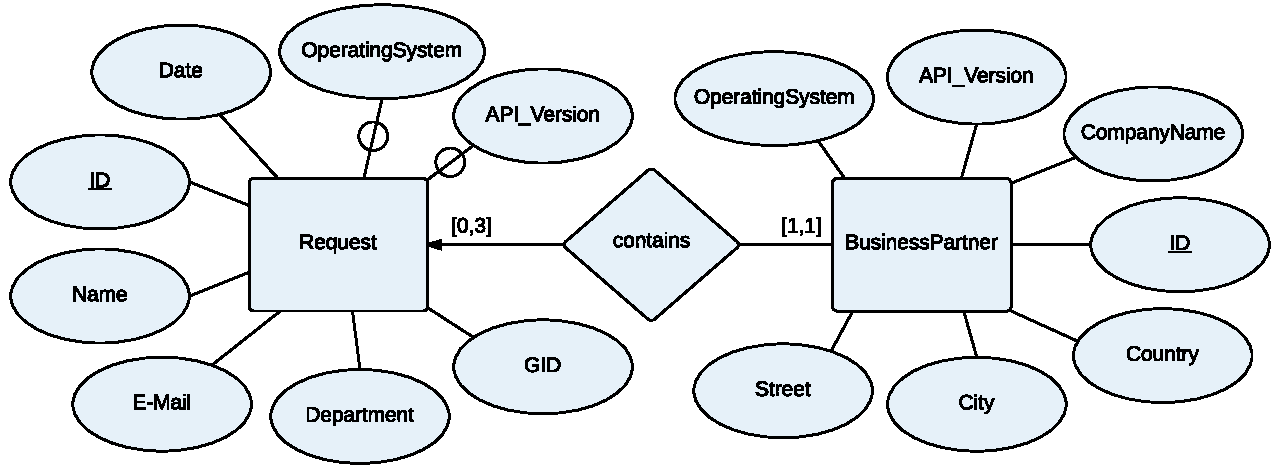
\includegraphics[width=\textwidth]{\figdir/er-model.pdf}
\end{subfigure}
\end{figure}

\begin{figure}[H]
\ContinuedFloat
\centering
\begin{subfigure}{\textwidth}
\caption{Zweiter Teil}
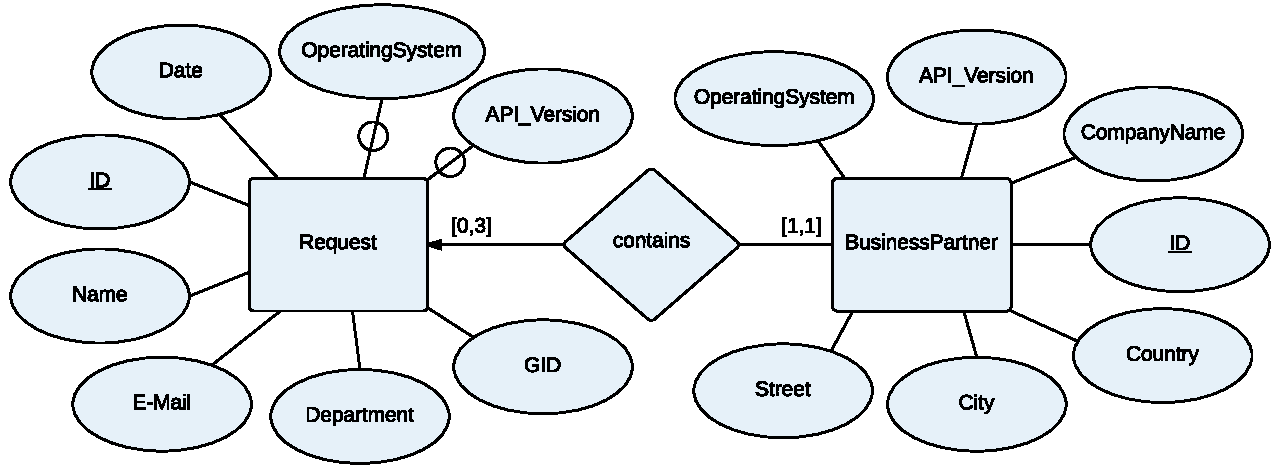
\includegraphics[width=\textwidth]{\figdir/er-model.pdf}
\end{subfigure}
\caption{Nochmal die gleiche Beispielgrafik}
\label{fig:workflow}
\end{figure}

So und jetzt viel Spaß mit \LaTeX!! Am anfang muss man zwar viel googlen, aber geht eigentlich relativ schnell. Könnt mich auch gerne fragen wenn irgendwas unklar ist.
